\hypertarget{self-interacting-dark-matter}{%
\chapter{Self-interacting dark
matter}\label{self-interacting-dark-matter}}

\hypertarget{introduction}{%
\section{Introduction}\label{introduction}}

Self-interacting dark matter (SIDM) was introduced in 2000 by Spergel
and Steinhardt~\cite{spergel_observational_2000}. The model was proposed as
a solution to the core-cusp and missing satellites problems, as the
addition of self-interactions was thought to have three primary effects
on the distribution of dark matter. 

\begin{enumerate}
    \item Self-interactions in regions of high density would cause dark matter
    particles to come unbound, reducing the density of halos primarily in
    their center region.  This would yield a cored density profile rather than
    a cuspy one, solving the core-cusp problem.

    \item It is also expected that interactions would yield a more isotropic
    velocity dispersion than seen in CDM as well as erase the typical triaxial
    ellipticity seen in halo shapes. In other words, SIDM halos should be more
    spherical, a testable prediction.

    \item Through the processes of isotropizing the velocity dispersion and
    reducing density in core regions, it was also expected that substructure
    would be greatly reduced, lowering the number of dwarf galaxies and
    thereby solving the missing satellites problem.
\end{enumerate}

One other feature of the model is that the dark matter scattering rate is
naturally dependent on the dark matter density. This means that one expects the
effects of self-interaction to be neglible toward the outermost radii of halos
and on larger scales, where $\Lambda$CDM predictions are consistent with
observations. As such, SIDM is able to successfully preserve the large-scale
successes of the $\Lambda$CDM model.

Shortly thereafter began a wave of numerical simulations to test these
predictions. The results of these simulations were mixed. Some were focused on
the evolution of galaxies and found confirmation of the predicted effects
(more strongly spherical shape, cored density profile)
like~\cite{burkert_structure_2000,dave_halo_2001}. Other simulations, like
cluster and cosmological simulations, seemed to show that SIDM would be
inconsistent with
observation~\cite{moore_collisional_2000,yoshida_collisional_2000,yoshida_weakly_2000}.

At the same time, constraints on the allowed self-interaction cross section
began being compiled, primarily from clusters. Given the lack of knowledge of
the mass of dark matter particles, cross section values are generally given as
cross section-to-mass ratios, denoted $\sigma/m$. We will use the term cross
section interchangeably with this. \cite{meneghetti_giant_2001}~used cluster
simulations to limit the allowable cross section to \(< 0.1\) cm\(^2\)/g.
Similarly, gravitational lensing data from the MS 2137-23 cluster was used by
\cite{miralda-escude_test_2002} to limit the cross section to \(< 10^{-25.5}\)
cm\(^2\)/GeV, approximately 0.02 cm\(^2\)/g. These cross sections were far too
small to solve the small-scale problems in galaxies, as simulations
like~\cite{dave_halo_2001} suggested the necessary cross section to be in the
range \(10^{-25}\) to \(10^{-23}\) cm\(^2\)/MeV (0.05 to 5 cm\(^2\)/g).

However, more recent simulations with higher resolution, better statistics,
and updated algorithms for considering self-interactions have relaxed many of
these constraints significantly, improving the viability of the model and once
again sparking interest in self-interactions. Examples
include~\cite{rocha_cosmological_2013,peter_cosmological_2013,zavala_constraining_2013,elbert_core_2015}.
These newer, better simulations revised the previous constraints and generally
show that cross sections on the order of $\sigma / m \sim 0.1$ to 5
cm$^2$/g are viable and consistent with observation. Of particular relevance
for this thesis is \cite{rocha_cosmological_2013}, which put forth a novel
method for computing the effects of self-interactions in N-body simulation.
See Subsection~\ref{self-interaction-in-simulation} for a discussion of their
method.

\cite{tulin_dark_2018} have distilled the relevant modern observational
constraints on the self-interaction cross section into a table. The data are
reproduced in Table~\ref{tab:constraints}. In particular, notice that the data
are consistent with a decaying cross section as the velocity scale increases.
Specifically, all small-scale data is consistent with a cross section of
$\gtrsim 0.5$ to 1 cm$^2$/g, but larger-scale data is consistent with a cross
section which is $\sim 0.1$ cm$^2$/g or smaller.  This rules out any particle
models we find with a velocity-independent cross section from being able to
solve the small-scale problems.  However, such models may serve as good
approximations in a régime where the cross section does not vary much.

\begin{table}
    \centering
    \begin{tabular}{lccl}\toprule
        & $\sigma / m$ & $v_{\text{rel}}$ &
        \\
        & (cm$^2$/g) & (km/s) & Observation
        \\ \midrule
        Cores in spiral galaxies
        & $\gtrsim 1$ & 30-200 & Rotation curves
        \\
        TBTF in Milky Way
        & $\gtrsim 0.6$ & 50 & Stellar dispersion
        \\
        TBTF in Local Group 
        & $\gtrsim 0.5$ & 50 & Stellar dispersion
        \\
        Cores in clusters 
        & $\sim 0.1$ & 1500 & Stellar dispersion, lensing
        % \\
        % \textit{Abell 3827 subhalo merger} 
        % & $\sim 1.5$ & 1500 & DM-galaxy offset
        % \\
        % \textit{Abell 520 cluster merger} 
        % & $\sim 1$ & 2000-3000 & DM-galaxy offset
        \\ \midrule
        Halo shape/ellipticity
        & $\lesssim 1$ & 1300 & Cluster lensing surveys
        \\
        Substructure mergers
        & $\lesssim 2$ & 500-4000 & DM-galaxy offset
        \\
        Merging clusters
        & $\lesssim$ few & 2000-4000 & Post-merger halo survival
        % \\
        % \textit{Bullet cluster} & $\lesssim 0.7$ & 4000 & Mass-to-light ratio
        \\ \bottomrule
    \end{tabular}
    \caption{%
        Observational constraints on the self-interaction cross section of
        dark matter. All listed observations are derived from sets of multiple
        systems. ``TBTF'' is the abbreviation for ``too-big-to-fail.'' This is
        an abridged reproduction of the table compiled
        by~\cite{tulin_dark_2018}. A distinction is made between ``positive
        observations'' (above the horizontal rule) and ``constraints'' (below
        the horizontal rule) by the original authors. References to the
        original papers are given therein.
    }
    \label{tab:constraints}
\end{table}

% todo add one of those plots that shows it changing slowly for galactic scales

\hypertarget{particle-physics-models}{%
\section{Particle physics models}\label{particle-physics-models}}

Given that very little is known conclusively about the particle physics
nature of dark matter, the introduction of the possibility of
self-interactions makes way for a wealth of rich new theories. We will
cover a few of the most popularly considered models below.

\hypertarget{self-coupled-scalar}{%
\subsection{Self-coupled scalar}\label{self-coupled-scalar}}

The first particle model that we consider is the simplest: a scalar
particle, $\varphi$, that interacts with itself through a two-to-two coupling.
This can be described by the Lagrangian
\begin{equation}
\mathcal{L}_{\text{int}} = -\frac{\lambda}{4!} \varphi^4.
\end{equation}
From the Lagrangian, we can read off the Feynman rule for a four-point
intersection to have the matrix element \(i\mathcal{M} = -i\lambda\), yielding
the two-to-two self-interaction differential cross section
\begin{equation}
\frac{d\sigma}{d\Omega} = \frac{\lambda^2}{64\pi^2 (4m^2)}.
\end{equation}
Integrating over the solid angle and dividing by two to account for identical
particles gives a total cross section
\begin{equation}
\sigma(\varphi\varphi\to\varphi\varphi) = \frac{\lambda^2}{128\pi m^2}.
\end{equation}
One can easily see that this cross section does not admit any kind of
velocity dependence. Thus, one could make this model consistent for a
small subset of scales (e.g. \(\sigma/m \sim 1\) cm\(^2\)/g for dwarf galaxy
scales), but then it would necessarily fail on other scales. This makes the
model viable only for analyses of limited scales where the cross section is
not expected to vary greatly, but it is generally infeasible as a solution to
the small-scale problems.

\hypertarget{light-mediator}{%
\subsection{Light mediator}\label{light-mediator}}

Perhaps the simplest model with a theory rich enough to solve all of the
observed problems is one wherein dark matter self-interactions are
mediated by a light particle. We will consider a model where dark matter
is represented by \(\chi\) and has mass \(m_\chi\), and the mediator
field is \(\phi\) with mass \(m_\phi\). This theory works with both
scalar and vector mediators, depending on what specific theory one wants
to consider. Perhaps the best motivated origin for such a model is one
where the dark matter particle is charged under a spontaneously broken
\(U(1)\) symmetry and the mediator arises as the corresponding gauge
boson~\cite{tulin_dark_2018}.

Such a model would have an interaction Lagrangian given by
\begin{equation}
\mathcal{L}_{\text{int}} =
\left\{ 
\begin{array}{cl}
    g_\chi \overline{\chi} \gamma^\mu \chi \phi_\mu
    & (\text{vector mediator}), \\
    g_\chi \overline{\chi} \chi \phi
    & (\text{scalar mediator}), \\
\end{array}
\right.
\end{equation}
where we let the coupling constant be \(g_\chi\). In the non-relativistic
limit, the interaction is well-approximated by the Yukawa potential~\cite{tulin_beyond_2013,tulin_resonant_2013}
\begin{equation}
V(r) = \pm \frac{\alpha_\chi}{r} e^{-m_\phi r},
\end{equation}
where \(\alpha_\chi \equiv g_\chi^2/4\pi\) is the dark fine structure
constant. The \(\pm\) will be set depending on whether the interaction is
attractive or repulsive. For a scalar \(\phi\), the potential is attractive
and the sign is \((-)\). For vector \(\phi\), the potential is attractive
\((+)\) for \(\chi\overline{\chi}\) scattering and repulsive \((-)\) for
\(\chi\chi\) and \(\overline{\chi}\overline{\chi}\) scattering.

Using the Yukawa potential, we can obtain the Born differential cross section
in the limit that \(\alpha_\chi m_\chi / m_\phi \ll 1\) to
be~\cite{tulin_dark_2018}
\begin{equation}
\frac{d\sigma}{d\Omega} = \frac{\alpha_\chi^2 m_\chi^2}{\left[
    m_\chi^2 v_{\text{rel}}^2 (1 - \cos\theta) / 2
    + m_\phi^2 \right]^2}.
\end{equation}
An important implication of this formula is that the mediator mass must be
positive, i.e. \(m_\phi > 0\). If instead \(m_\phi = 0\), we would then find
that \( d\sigma/d\Omega \propto v_{\text{rel}}^{-4}\), which is far too strong
at small velocities to admit a solution which is consistent with observations.
A small but nonzero mediator mass \(m_\phi\), on the other hand, allows us to
``soften'' this velocity-dependence to admit a more consistent model.

While quite simple, it has been shown in~\cite{tulin_resonant_2013} that it is
possible for this model to simultaneously accommodate all important
observations and solve the small scale problems.

\hypertarget{strong-interactions}{%
\subsection{Strong interactions}\label{strong-interactions}}

Some of the richest theories for self-interacting dark matter candidates that
one can consider are non-Abelian gauge theories where the dark matter
candidates arise as composite bound states. In these theories, the
self-interaction manifests as a strong interaction.

The motivation for considering such a model comes from our experience with QCD
and the visible sector~\cite{kribs_review_2016}. For a dark matter model to be
a good candidate, it must be stable over the lifetime of the Universe and be
neutral under Standard Model phenomena. Further, we desire models in which the
particles exhibit strong self-interactions. These are all properties exhibited
by particles in the visible sector under QCD, so it makes sense to consider a
similar theory to describe our dark matter candidate. However, we do not
necessarily know the gauge group or particle properties of dark matter,
leaving us a great freedom to vary the model significantly. Many of the
resulting models thus have interesting and unique new physics, though these
details are greatly model-dependent.

The primary free parameters of models of this kind are the confinement scale
\(\Lambda\) (different from the cosmological constant), and the dark quark
mass(es). In the event that our ``dark QCD'' contains no analogue to
electromagnetic/weak interactions, meson-like bound states of the dark quarks
could be stable~\cite{cline_composite_2014}. These mesons can be classified as
loosely pion-like, where \(m \ll \Lambda\), or quarkonium-like, where \(m \gg
\Lambda\)~\cite{kribs_review_2016}. There are several proposed models for each
of these scenarios; one of the more well-known is the strongly-interacting
massive particle, or SIMP, where the dark matter candidate is pion-like and
many non-Abelian theories are possible.

Our non-Abelian model may instead look quite similar to visible QCD, wherein
the primary stable bound states are baryonic in nature.
In~\cite{kribs_review_2016}, it is noted that the advantage of such models is
that ``dark matter is automatically sufficiently stable, and no further
ultraviolet model-building is needed.'' One such dark baryon model is
``Stealth Dark Matter,'' proposed by the LSD collaboration, which is a scalar
dark baryon under a confining \(SU(4)\) theory. This theory is named
\emph{stealth} dark matter because it is found that the baryons are safe from
direct detection, though it does predict a spectrum of lighter meson particles
that would be possible to detect at colliders~\cite{kribs_review_2016}.

The third class of candidate particles that has received attention are dark
glueballs. Glueballs are bound states of only gluons and are predicted to
exist in QCD, but are very difficult to detect. Dark glueballs would then be
bound states of dark gluons. Such a model is possible if all the dark fermions
in the theory have masses significantly larger than \(\Lambda\). In this case,
glueballs may become stable under an accidental symmetry like baryons,
allowing them to be the primary dark matter candidate.

The observables that could result from the above considerations are as diverse
as the models themselves. One aspect of these models that we have not
considered is what the interactions with the Standard Model could look like.
Some models predict the dark matter candidate to be neutral under Standard
Model interactions, but its constituents to be charged. In such a case, the
model would have a coupling to the photon, and it would be possible to
directly detect the particle. We may also consider the case where our theory
predicts fundamental fermions. It is plausible that these fermions would
obtain at least part of their mass through a coupling to the Higgs boson,
again providing a mechanism by which we could directly detect the particles.
Kribs and Neil provide more details of these observables, as well as
collider-specific results, in~\cite{kribs_review_2016}.

\hypertarget{analytic-description-with-baryons}{%
\section{Analytic description of mass distributions}\label{analytic-description-with-baryons}}

The most obvious manifestation of dark matter self-interaction is in its
effects on astrophysical mass distributions.  As such, an understanding of the
particle physics properties of dark matter, like the self-interaction cross
section, will require the ability to analytically describe and understand the
impact of these properties on astrophysical observables.  To this end, we
present the Jeans approach, an analytic method for deriving the equilibrium
distribution of self-interacting dark matter in the presence of baryons,
following closely the work of Kaplinghat et al.~\cite{kaplinghat_tying_2014}.

The discussion begins with the time-independent Jeans equation, e.g.~Equation
4.209 of~\cite{binney_galactic_2008}, which is 
\begin{equation}
    - \overline{v}_j \frac{\partial (\nu \overline{v}_i)}{\partial r_i} 
    = - \nu \frac{\partial \Phi_{\text{tot}}}{\partial r_j} 
    - \frac{\partial (\nu \sigma_{ij}^2)}{\partial r_j},
\end{equation}
where $\nu$ is the number density of dark matter, $\overline{\mathbf{v}}$ is
the mean velocity of dark matter particles, and $\Phi_{\text{tot}}$ is the
total gravitational potential.  We assume that the velocity dispersion is a
constant $\sigma_0$, and that the time required for dark matter to attain
equilibrium through self-scattering is long, which allows us to neglect the
self-scattering term (on the left side of the equation).  We can also write
the equation in terms of the mass density $\rho$ instead of the number density
$\nu$, as $\rho \propto \nu$ since each dark matter particle will have the
same mass.  With these assumptions, the equation becomes
\begin{equation}
    \rho \nabla_r \Phi_{\text{tot}}(\mathbf{r}) + \sigma_0^2 \nabla_r
    \rho(\mathbf{r}) = 0.
\end{equation}
We can divide through by $\rho$ and recognize that $\nabla \rho / \rho = \nabla
(\ln \rho)$, yielding 
\begin{equation}
    \sigma_0^2 \nabla_r (\ln \rho(\mathbf{r})) + \nabla_r
    \Phi_{\text{tot}}(\mathbf{r}) = 0.
\end{equation}
We then take the derivative of the entire equation.  At this point, we can
introduce a length scale $r_0$ and corresponding dimensionless length
$\mathbf{x} = \mathbf{r} / r_0$.
\begin{equation}
    \sigma_0^2 \nabla_x^2 (\ln \rho(\mathbf{x})) + \nabla_x^2
    \Phi_{\text{tot}}(\mathbf{x}) = 0.
\end{equation}
Now we can use Poisson's equation, $\nabla_x^2 \Phi_{\text{tot}}(\mathbf{x}) =
r_0^2 \nabla_r^2 \Phi_{\text{tot}}(\mathbf{r}) = 4 \pi G r_0^2
\rho_{\text{tot}}(\mathbf{r})$.  Letting the dark matter density be $\rho$ and
the baryon density be $\rho_B$, this yields
\begin{equation}
    \nabla_x^2 (\ln \rho(\mathbf{x})) + (4 \pi G r_0^2/\sigma_0^2) \left[ \rho_B (\mathbf{x}) + \rho(\mathbf{x}) \right] = 0.
\end{equation}
Now, for convenience, we introduce a function $h(\mathbf{x}) = \ln
\rho(\mathbf{x})$ such that $\rho(\mathbf{x}) = \rho_0 \exp(h(\mathbf{x}))$.
The result is given by Equation 1 in~\cite{kaplinghat_tying_2014}, here
\begin{equation}
\nabla_x^2 h(\mathbf{x}) + (4\pi G r_0^2/\sigma_0^2)
\left[\rho_B(\mathbf{x}) + \rho_0 \exp\left(h(\mathbf{x})\right)\right] = 0.
\end{equation}

As a simple test of this equation, we can consider the case where
baryonic matter dominates. Then, the $\exp(h)$ term can be neglected,
yielding
\begin{equation}
\nabla_x^2 h(\mathbf{x}) + (4\pi G r_0^2/\sigma_0^2) \rho_B(\mathbf{x}) = 0.
\end{equation}
We use Poisson's equation to rewrite $\rho_B$ in terms of the baryonic
gravitational potential $\Phi_B$,
\begin{equation}
\nabla_x^2 h(\mathbf{x}) + \frac{1}{\sigma_0^2} \nabla_x^2 \Phi_B(\mathbf{x}) = 0.
\end{equation}
Integrating over $x$ gives the solution 
\begin{equation}
h(\mathbf{x}) = \frac{1}{\sigma_0^2} \left(\Phi_B(0) - \Phi_B(\mathbf{x})\right),
\end{equation}
which corresponds to a dark matter density of 
\begin{equation}
\rho(\mathbf{x}) = \rho_0 \exp\left[\frac{1}{\sigma_0^2} 
\left(\Phi_B(0) - \Phi_B(\mathbf{x})\right) \right].
\end{equation}
The authors then recommend defining the core radius as the radius at
which the density is half the initial density, \(\rho_0 / 2\). Such a position
would give \(h(\mathbf{r}_c) = -\ln 2\), or
\begin{equation}
\Phi_B(0) - \Phi_B(\mathbf{r}_c) = -\sigma_0^2 \ln 2.
\end{equation}
Thus, the core size would depend only on the baryonic potential in the case
where it dominates, which follows from these assumptions but stands in marked
contrast to observation, where the baryonic contribution does not dominate.

At this point, the authors make the move to consider the spherically symmetric
case. To do so, they approximate the Milky Way baryon distribution, $\rho_B$, by
a Hernquist profile whose spherical enclosed mass distribution approximates
the true enclosed mass distribution. The Hernquist density profile is given by 
\begin{equation}
\rho_B(r) = \frac{\rho_{B0}}{(r/r_0) (1 + r/r_0)^3},
\end{equation}
corresponding to a gravitational potential of 
\begin{equation}
\Phi_B(r) = - \frac{G M_B}{r + r_0},
\end{equation}
where $M_B$ is the total mass of baryons in the Milky Way. The free parameters
can be set by finding $r_0$ and $\Phi_B(0)$ such that the circular velocity
$V_B(r_0)^2 = - \Phi_B(0) / 4$ matches observation. The authors give
$\sqrt{-\Phi_B(0)} = 365$ km/s and $r_0 = 2.7$ kpc to be a good fit. We can thus
find the core size by solving
\begin{equation}
-\sigma_0^2 \ln 2 = \Phi_B(0) - \Phi_B(r_c) = \Phi_B(0) \left(1 - \frac{1}{1 + r_c/r_0}\right),
\end{equation}
which gives 
\begin{equation}
r_c 
\approx \frac{r_0 \sigma_0^2 \ln 2}{-\Phi_B(0)} 
= \frac{r_0 \sigma_0^2 \ln 2}{4 V_B(r_0)^2}.
\end{equation}
For a typical value of $\sigma_0$, on the order of 150 km/s, we thus obtain 
\begin{equation}
r_c \approx 0.3 \text{ kpc} 
\left(\frac{r_0}{2.7 \text{ kpc}}\right)
\left(\frac{\sigma_0}{150 \text{ km/s}}\right)^2
\left(\frac{183 \text{ km/s}}{V_B(r_0)}\right)^2,
\end{equation}
which is quite small.

Let's continue under the assumption that the Milky Way is spherically symmetric
and that its baryon profile can be approximated by a Hernquist profile, but drop
the assumption that baryons dominate the potential. To begin, we will rewrite
the Jeans equation in a spherically symmetric system. First, note that
\begin{equation}
\frac{4\pi G r_0^2}{\sigma_0^2} \rho_B(x)
= \frac{1}{\sigma_0^2} \nabla_x^2 \Phi_B(x)
= \nabla_x^2 \left( \frac{\Phi_B(0)}{\sigma_0^2} \frac{1}{1 + x} \right).
\end{equation}
Thus, we can rewrite the Jeans equation as 
\begin{align}
0
&= \nabla_x^2 \left( h(x) + \frac{\Phi_B(0)}{\sigma_0^2} \frac{1}{1 + x} \right)
    + \frac{4\pi G \rho_0 r_0^2}{\sigma_0^2} e^{h(x)} \\
&= \frac{1}{x^2} \frac{\partial}{\partial x} 
    \left[ x^2 \frac{\partial}{\partial x} 
    \left( h(x) + \frac{\Phi_B(0)}{\sigma_0^2} \frac{1}{1 + x} \right) \right]
    + \frac{4\pi G \rho_0 r_0^2}{\sigma_0^2} e^{h(x)}.
\end{align}
We now introduce a new dimensionless variable, $y = x/(1+x)$. Substituting it in
yields
\begin{equation}
\frac{(1-y)^4}{y^2} \frac{\partial}{\partial y} 
    \left[ y^2 \frac{\partial}{\partial y}
    \left( h(y) + \frac{\Phi_B(0)}{\sigma_0^2} (1 - y) \right) \right]
    + \frac{4\pi G \rho_0 r_0^2}{\sigma_0^2} e^{h(y)} = 0.
\end{equation}
Simplifying, we then obtain 
\begin{equation}
\frac{1}{y^2} \frac{\partial}{\partial y} \left( 
    y^2 \frac{\partial h}{\partial y} \right) 
    - \frac{2 \Phi_B(0)}{\sigma_0^2} \frac{1}{y}
    + \frac{4\pi G \rho_0 r_0^2}{\sigma_0^2} 
    \frac{e^{h(y)}}{(1-y)^4} = 0.
\end{equation}
The authors recommend that this equation be simplified by letting $a_0$ be the
coefficient for the $\exp(h(y))$ term and $a_1 = - \Phi_B(0) / \sigma_0^2$.
The boundary conditions imposed on the equation are then $h(0) = 0$ and $h'(0)
= -a_1$, which enforce a core in the center.

We can then solve this equation approximately within the core by approximating
the third term by $a_0$, equivalent to setting $y = 0$ in this term alone. The
resulting equation has approximate solution 
\begin{equation}
    h(y) \approx -a_1 y - \frac{1}{6} a_0 y^2.
\end{equation}
In the case that baryons dominate, $a_1 \gg a_0$ and the $y^2$ term becomes
negligible. The core radius then is given by the solution to 
\begin{equation}
    \frac{\ln 2}{a_1} = \frac{r_c}{r_0 + r_c},
\end{equation}
which is 
\begin{equation}
    r_c = r_0 \frac{\ln 2}{a_1 - \ln 2} \approx 
    \frac{r_0 \sigma_0^2 \ln 2}{-\Phi_B(0)},
\end{equation}
the same result as we derived before. In the case that dark matter dominates,
$a_0 \gg a_1$ and the $y$ term becomes negligible. The core radius is given by
the solution to 
\begin{equation}
    \frac{6 \ln 2}{a_0} = \left(\frac{r_c}{r_0 + r_c}\right)^2,
\end{equation}
which is 
\begin{equation} \label{eq:core_dm_dom}
    r_c = r_0 \frac{\sqrt{6\ln 2}}{a_0 - \sqrt{6\ln 2}} \approx 
    r_0 \sqrt{6 \ln 2 / a_0} = \sqrt{\frac{3 \ln 2\, \sigma_0^2}{2 \pi G \rho_0}}.
\end{equation}
The authors reference an SIDM simulation of a Milky Way-sized halo with a
resulting inner density of approximately 2.2 GeV $c^{-2}$ cm$^{-3}$. In the dark
matter dominated limit, we thus estimate the core size to be approximately 5.5
kpc, which is consistent with simulation. 

For the case where neither baryons nor dark matter dominate, the authors give
the following result for the core size
\begin{equation} \label{eq:core_size}
    r_c \approx r_0 \frac{\sqrt{1 + \frac{2 \ln 2\, a_0}{3 a_1^2}} - 1}{
        1 + \frac{a_0}{3 a_1} - \sqrt{1 + \frac{2 \ln 2\, a_0}{3 a_1^2}} 
    }.
\end{equation}
However, we have potentially a family of solutions parameterized by $a_0$ and
$a_1$. As a criterion for consistent selection, then, the authors adopt the
following convention. Let $r_1$ be the radius at which the average dark matter
particle has undergone one interaction. We choose the values of $a_0$ and
$a_1$ such that the mass and total energy within $r_1$ match the values that
one would have had in the absence of self-interactions. To compare against
``the absence of self-interactions,'' one can look at, for example, an NFW
profile that approximately fits the considered galaxy.

For the Milky Way, we can consider the self-interaction cross section required
for $r_1$ to be approximately the solar radius, 8.5 kpc. The local dark matter
density is known to be approximately 0.2 GeV $c^{-2}$ cm$^{-3}$. We can also
estimate the age of the Milky Way to be 10 Gyr. Thus, we expect the average
number of scatterings to be approximately
\begin{equation}
    \left( 0.2 \text{ GeV $c^{-2}$ cm$^{-3}$} \right)
    \left( 150 \text{ km/s} \right)
    \left( \sigma/m \right)
    \left( 10 \text{ Gyr} \right).
\end{equation}
A self-interaction cross section of about $\sigma/m = 1$ barn/GeV (0.56
cm$^2$/g) sets this to one scattering event per particle. As we have seen, this
cross section is consistent with observations on the scales of galaxies and is
capable of solving the small-scale problems.

The authors specifically consider values of $\sigma_0$, $\rho_0$, and $r_1$
that approximate the Milky Way in the case that the no-self-interaction halo is
well described by an NFW profile. They find that $r_1 = 15$ kpc, $\sigma_0 =
165$ kpc, $\sigma / m = 1$ barn/GeV, and $\rho_0 = 14$ GeV $c^{-2}$ cm$^{-3}$
gives a good fit. When plugged into Equation~\ref{eq:core_size}, this yields an
expected core size of 0.43 kpc. The resulting density profiles are shown in
Figure~\ref{fig:sidm_expected_density}. In particular, note that the dashed red
curve (SIDM analog to the standard NFW Milky Way) attains half its central
density at approximately 0.5 kpc, in line with the analytic expectation.

\begin{figure}
    \centering
    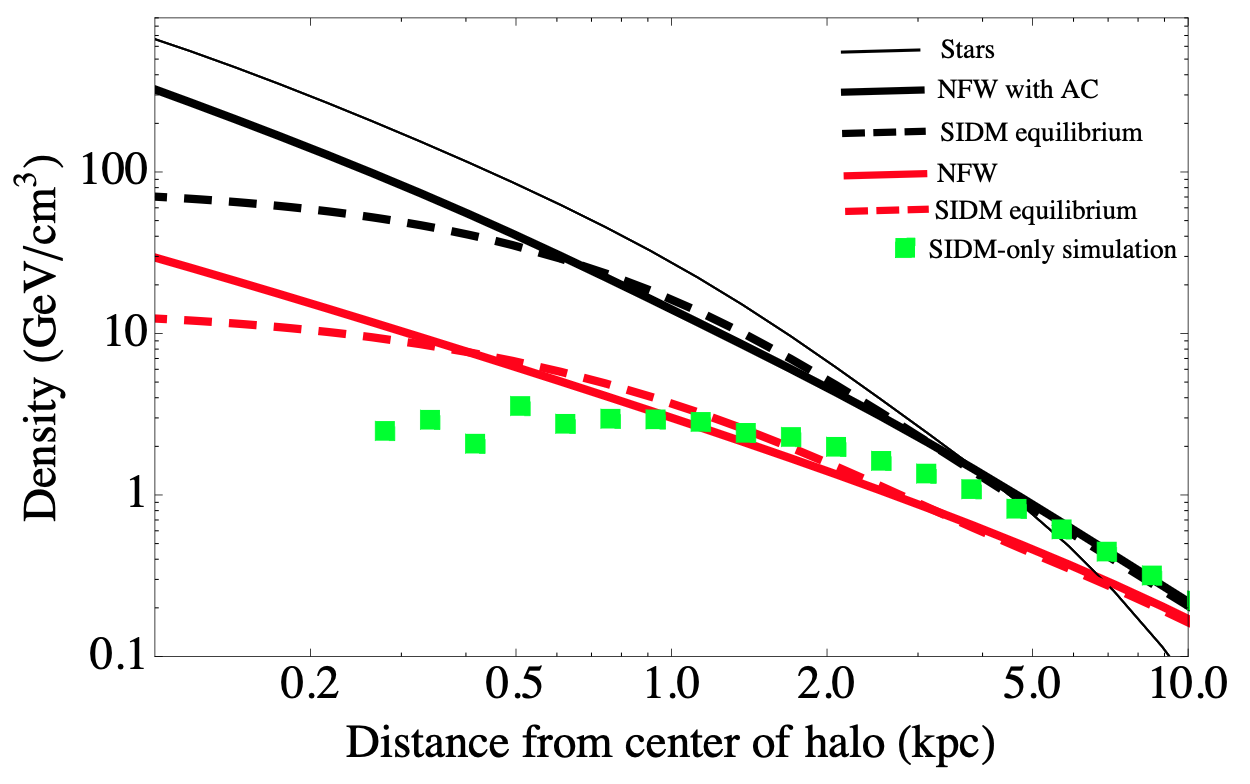
\includegraphics[width=0.65\linewidth]{figs/kaplinghat_sidm_density.png}
    \caption{%
        Mass density distributions for a Milky Way-sized halo. The green boxes
        show the result of a dark matter-only SIDM simulation. The thick solid
        lines show NFW distributions, both adiabatically contracted (black)
        and not (red). (We focus only on the non-adiabatically contracted case
        in this study.) The dashed lines show the corresponding analytic SIDM
        profiles expected from the results of the Jeans equation-based
        formalism. This figure is reproduced from Figure 1
        of~\cite{kaplinghat_tying_2014}.
    }
    \label{fig:sidm_expected_density}
\end{figure}


\hypertarget{self-interaction-in-simulation}{%
\section{Self-interaction in simulation}\label{self-interaction-in-simulation}}

In this work, we will be exploring the introduction of self-interaction in
predictions about the infall of the Sagittarius dwarf galaxy and,
specifically, the formation of its stream. This is done through the use of
N-body simulations. As such, we present a description of how these
self-interactions are modeled in simulation. We choose to use
GIZMO~\cite{hopkins_new_2015} for our simulations, and the implementation of
self-interactions therein is the one described
by~\cite{rocha_cosmological_2013}. Much of the following discussion comes in
large part from~\cite{rocha_cosmological_2013}.

In our simulation, we consider some number of ``macro-particles,'' each
of which represents an ensemble of dark matter particles, or a patch of the
dark matter phase-space density. We let each macro-particle have mass
\(m_p\), and we keep this mass consistent across all dark matter
macro-particles. Since we consider the macro-particle as representing a
patch of the phase-space density, we consider its position to be
centered at some point \(\mathbf{x}\) but spread out according to a
kernel \(W(r,h)\). Here, \(r\) is the distance from the center of the
macro-particle and \(h\) is a smoothing length.  In
GADGET-2~\cite{springel_cosmological_2005}, from which GIZMO is built and
inherits its implementation of this algorithm, the kernel is given by
\begin{equation}
W(r,h) = \frac{8}{\pi h^3} \left\{ 
    \begin{array}{ll}
        1 - 6 (r/h)^2 + 6 (r/h)^3 & 0 \leq r/h \leq 1/2, \\
        2 (1 - r/h)^3 & 1/2 < r/h \leq 1, \\
        0 & r/h > 1.
    \end{array}
\right.
\end{equation}
The smoothing length in GIZMO is fixed and on the order of $10$ pc.  The
velocity of the macro-particle is taken to instead be a delta function, such
that the macro-particles have a single defined velocity.

When the patches represented by two macro-particles overlap, we can
compute the interaction rate between them. The rate of scattering of a
macro-particle \(j\) off a target particle \(i\) is given by
\begin{equation}
\Gamma(i|j) = (\sigma/m) m_p |\mathbf{v}_i - \mathbf{v}_j| g_{ji},
\end{equation}
where \(\sigma/m\) is the familiar cross section to mass ratio and
\(g_{ij}\) is a number density factor whose purpose is account for the
overlap of the two macro-particles' smoothing kernels. It is given by
\begin{equation}
g_{ji} = \int_{0}^{h} d^3 \mathbf{x}' \, W(|\mathbf{x}'|, h) \, 
W(|\delta \mathbf{x}_{ji} + \mathbf{x}'|, h),
\end{equation}
with \(\delta \mathbf{x}_{ji}\) the displacement vector between the
macro-particle positions.

Over the course of a time step \(\delta t\), the probability of an
interaction of macro-particle \(j\) off target macro-particle \(i\) is
given by 
\begin{equation}
P(i|j) = \Gamma(i|j) \, \delta t.
\end{equation}
The total probability
of interaction between these two particles in this time step, then,
would be the average of the two directed probabilities, i.e.
\begin{equation}
P_{ij} = \tfrac{1}{2} \left( P(i|j) + P(j|i) \right).
\end{equation}
To actually
represent the interaction, then, one draws a random number and adjusts
the velocities of the particles if the number lies below the
probability. The velocities are adjusted in a manner consistent with an
elastic scattering which is isotropic in the center of mass frame.

More details are presented in~\cite{rocha_cosmological_2013}, including the
derivation of the scattering rate formula from the Boltzmann equation. We use
the implementation which is packaged with the publicly-available
GIZMO~\cite{hopkins_new_2015} simulation suite.
